% PRL look and style (easy on the eyes)
\documentclass[aps,pre,twocolumn,nofootinbib,superscriptaddress,linenumbers,11point]{revtex4-1}
% Two-column style (for submission/review/editing)
%\documentclass[aps,prl,preprint,nofootinbib,superscriptaddress,linenumbers]{revtex4-1}

%\usepackage{palatino}

% Change to a sans serif font.
\usepackage{sourcesanspro}
\renewcommand*\familydefault{\sfdefault} %% Only if the base font of the document is to be sans serif
\usepackage[T1]{fontenc}
%\usepackage[font=sf,justification=justified]{caption}
\usepackage[font=sf]{floatrow}

% Rework captions to use sans serif font.
\makeatletter
\renewcommand\@make@capt@title[2]{%
 \@ifx@empty\float@link{\@firstofone}{\expandafter\href\expandafter{\float@link}}%
  {\textbf{#1}}\sf\@caption@fignum@sep#2\quad
}%
\makeatother

\usepackage{listings} % For code examples
\usepackage[usenames,dvipsnames,svgnames,table]{xcolor}

\usepackage{minted}

\usepackage{amsmath}
\usepackage{amssymb}
\usepackage{graphicx}
%\usepackage[mathbf,mathcal]{euler}
%\usepackage{citesort}
\usepackage{dcolumn}
\usepackage{boxedminipage}
\usepackage{verbatim}
\usepackage[colorlinks=true,citecolor=blue,linkcolor=blue]{hyperref}


% The figures are in a figures/ subdirectory.
\graphicspath{{figures/}}

% italicized boldface for math (e.g. vectors)
\newcommand{\bfv}[1]{{\mbox{\boldmath{$#1$}}}}
% non-italicized boldface for math (e.g. matrices)
\newcommand{\bfm}[1]{{\bf #1}}          

%\newcommand{\bfm}[1]{{\mbox{\boldmath{$#1$}}}}
%\newcommand{\bfm}[1]{{\bf #1}}
%\newcommand{\expect}[1]{\left \langle #1 \right \rangle}                % <.> for denoting expectations over realizations of an experiment or thermal averages

% Define some useful commands we will use repeatedly.
\newcommand{\T}{\mathrm{T}}                                % T used in matrix transpose
\newcommand{\tauarrow}{\stackrel{\tau}{\rightarrow}}       % the symbol tau over a right arrow
\newcommand{\expect}[1]{\langle #1 \rangle}                % <.> for denoting expectations over realizations of an experiment or thermal averages
\newcommand{\estimator}[1]{\hat{#1}}                       % estimator for some quantity from a finite dataset.
\newcommand{\code}[1]{{\tt #1}}

% vectors
\newcommand{\x}{\bfv{x}}
\newcommand{\y}{\bfv{y}}
\newcommand{\f}{\bfv{f}}

\newcommand{\bfc}{\bfm{c}}
\newcommand{\hatf}{\hat{f}}

%\newcommand{\bTheta}{\bfm{\Theta}}
%\newcommand{\btheta}{\bfm{\theta}}
%\newcommand{\bhatf}{\bfm{\hat{f}}}
%\newcommand{\Cov}[1] {\mathrm{cov}\left( #1 \right)}
%\newcommand{\Ept}[1] {{\mathrm E}\left[ #1 \right]}
%\newcommand{\Eptk}[2] {{\mathrm E}\left[ #2 \,|\, #1\right]}
%\newcommand{\T}{\mathrm{T}}                                % T used in matrix transpose
%\newcommand{\conc}[1] {\left[ \mathrm{#1} \right]}

\newcommand{\pyitc}{\url{http://www.simtk.org/home/bayesian-itc}} % URL of pyITC project homepage

%%%%%%%%%%%%%%%%%%%%%%%%%%%%%%%%%%%%%%%%%%%%%%%%%%%%%%%%%%%%%%%%%%%%%%%%%%%%%%%%
% DOCUMENT
%%%%%%%%%%%%%%%%%%%%%%%%%%%%%%%%%%%%%%%%%%%%%%%%%%%%%%%%%%%%%%%%%%%%%%%%%%%%%%%%

\begin{document}

%%%%%%%%%%%%%%%%%%%%%%%%%%%%%%%%%%%%%%%%%%%%%%%%%%%%%%%%%%%%%%%%%%%%%%%%%%%%%%%%
% TITLE
%%%%%%%%%%%%%%%%%%%%%%%%%%%%%%%%%%%%%%%%%%%%%%%%%%%%%%%%%%%%%%%%%%%%%%%%%%%%%%%%

\title{A simple method for automated equilibration detection in molecular simulations}

\author{John D. Chodera}
 \thanks{Corresponding author}
 \email{john.chodera@choderalab.org}
 \affiliation{Computational Biology Program, Sloan Kettering Institute, Memorial Sloan Kettering Cancer Center, New York, NY 10065}

\date{\today}

%%%%%%%%%%%%%%%%%%%%%%%%%%%%%%%%%%%%%%%%%%%%%%%%%%%%%%%%%%%%%%%%%%%%%%%%%%%%%%%%
% ABSTRACT
%%%%%%%%%%%%%%%%%%%%%%%%%%%%%%%%%%%%%%%%%%%%%%%%%%%%%%%%%%%%%%%%%%%%%%%%%%%%%%%%

\begin{abstract}

Molecular simulations intended to compute equilibrium properties are often initiated from configurations that are highly atypical of equilibrium samples, a practice which can generate a distinct initial transient in mechanical observables computed over the timecourse of the simulation.
Traditional practice in simulation data analysis recommends this initial portion be discarded to \emph{equilibration}, but no simple, general, and automated procedure for this process exists.
Here, we suggest a conceptually simple, automated procedure that does not make strict assumptions about the distribution of the observable of interest, in which the equilibration region is chosen to maximize the number of effectively uncorrelated samples in the production portion used to compute equilibrium averages.
We present a simple reference implementation of the procedure in Python, and demonstrate its utility on both synthetic and real simulation data.\\

% KEYWORDS
\emph{Keywords: molecular dynamics (MD); Metropolis-Hastings; Monte Carlo (MC); Markov chain Monte Carlo (MCMC); equilibration; timeseries analysis; statistical inefficiency; integrated autocorrelation time}

\end{abstract}

\maketitle

%%%%%%%%%%%%%%%%%%%%%%%%%%%%%%%%%%%%%%%%%%%%%%%%%%%%%%%%%%%%%%%%%%%%%%%%%%%%%%%%
% INTRODUCTION
%%%%%%%%%%%%%%%%%%%%%%%%%%%%%%%%%%%%%%%%%%%%%%%%%%%%%%%%%%%%%%%%%%%%%%%%%%%%%%%%

\section*{Introduction}
\label{section:introduction}

Molecular simulations use Markov chain Monte Carlo (MCMC) techniques~\cite{jun-s-liu:mcmc} to sample configurations $x$ from an equilibrium distribution $\pi(x)$, either exactly (using Monte Carlo methods such as Metropolis-Hastings) or approximately (using molecular dynamics integrators without Metropolization)~\cite{sivak:2013:prx:vvvr}.

Due to the sensitivity of the equilibrium distribution $\pi(x)$ to small perturbations in configuration $x$ and the difficulty of producing sufficiently good guesses of typical equilibrium configurations, these molecular simulations are often started from highly atypical initial conditions.
For example, simulations of biopolymers might be initiated from a fully extended conformation unrepresentative of behavior in solution, or a geometry derived from a fit to diffraction data collected from a cryocooled crystal; 
solvated systems may be prepared by periodically replicating a small solvent box equilibrated under different conditions, yielding atypical densities and solvent structure; 
liquid mixtures or lipid bilayers may be constructed by using methods that fulfill spatial constraints (e.g.~PackMol~\cite{martinez:jctc:2009:packmol}) but create locally aytpical geometries, requiring long simulation times to relax to typical configurations.

As a result, traditional practice in molecular simulation has recommended some initial portion of the trajectory be discarded to \emph{equilibration} (also called \emph{burn-in}\footnote{The term \emph{burn-in} comes from the field of electronics, in which a short ``burn-in'' period is used to ensure that a device is free of faulty components---which often fail quickly---and is operating normally~\cite{crc-mcmc-handbook}.} in the MCMC literature~\cite{crc-mcmc-handbook}).
While this practice is strictly unnecessary for the time-average of quantities of interest to eventually converge to the desired expectations~\cite{geyer:burn-in-unnecessary,crc-mcmc-handbook}, it nevertheless often allows the practitioner to avoid impractically long run times to eliminate the bias in computed properties in finite-length simulations induced by atypical initial starting conditions.

% Liquid argon example
% JDC: Should we use TIP3P water instead?
As an illustrative example, consider the computation of the average density of liquid argon under a given set of reduced temperature and pressure conditions Figure~\ref{figure:burn-in-example}.
To initiate the simulation, an initial dense liquid geometry at reduced density $\rho^* \equiv \rho \sigma^3 = 0.960$ was prepared and subjected to local energy minimization.
Figure~\ref{figure:burn-in-example} (top) depicts the relaxation behavior of 100 simulations initiated from the same configuration with different random initial velocities and integrator random number seeds.
The average (black line) and standard deviation (shaded grey) shows that all realizations of this simulation show a characteristic relaxation behavior away from the initial density toward a new equilibrium density.
The expectation of the running average of the density over many realizations of this procedure ({Figure~\ref{figure:burn-in-example}, bottom}) significantly deviates from the actual expectation, which would lead to biased estimates unless simulations were sufficiently long to eliminate this starting point dependent bias.
Note that this significant bias is present because the \emph{same} atypical starting condition is used for every realization of this simulation process.

Consider successively sampled configurations $x_t$ from a molecular simulation, with $t = 1, \ldots, T$.
We presume we are interested in computing the expectation $\expect{A} \equiv \int dx \, A(x) \, \pi(x)$ of a mechanical property $A(x)$.
For convenience, we will refer to the timeseries $a_t \equiv A(x_t)$, with $t = 0$.
The estimator $\hat{A} \approx \expect{A}$ constructed from the entire dataset is given by
\begin{eqnarray}
\hat{A}_{[1,T]} \equiv \frac{1}{T} \sum_{t=1}^T a_t . \label{equation:time-average}
\end{eqnarray}
While $\lim_{T \rightarrow \infty} \hat{A}_{[1,T]} = \expect{A}$ for an infinitely long simulation\footnote{We note that this equality only holds for simulation schemes that sample from the true equilibrium distribution $\pi(x)$, such as Metropolis-Hastings Monte Carlo or Metropolized integration schemes. Molecular dynamics simulations utilizing finite timestep integration without Metropolization will produce averages that may deviate from the true expectation $\expect{A}$~\cite{deviation}.}, the bias in $\hat{A}_{[1,T]}$ may be significant in a simulation of finite length $T$.

By discarding samples $t < t_0$ to equilibration, we hope to eliminate the initial transient and provide a less biased estimate of $\expect{A}$,
\begin{eqnarray}
\hat{A}_{[t_0,T]} \equiv \frac{1}{T-t_0+1} \sum_{t=t_0}^T a_t . \label{equation:production-time-average} 
\end{eqnarray}
We can quantify the bias in an estimator $\hat{A}$ by the expected error $\delta^2 \hat{A}$,
\begin{eqnarray}
\delta^2 \hat{A} &\equiv& E_{x_0} \left| \left( \hat{A} - \expect{A} \right)^2 \right] . \label{equation:error} 
\end{eqnarray}
where $E_{x_0}[\cdot]$ denotes the expectation over independent realizations of the simulation from the same initial configuration $x_0$ but different initial velocities and random number seeds.

Here, we concern ourselves with this question: 
Is there a simple approach to choosing an optimal equilibration time $t_0$ that provides an improved estimate $\hat{A}_{[t_0,T]}$, such that $\delta^2 \hat{A}_{[t_0,T]} < \delta^2 \hat{A}_{[1,T]}$?
We note that, for cases in which the simulation is not long enough to reach equilibrium, no choice of $t_0$ will eliminate bias completely; the best we can hope for is to minimize this bias.

While several automated methods for selecting the equilibration time $t_0$ have been proposed, these approaches have shortcomings that have greatly limited their use.
The reverse cumulative averaging method~\cite{yang-karplus:2004:jcp:reverse-cumulative-averaging}, for example, uses a statistical test for normality to determine the point before which which the observable timeseries deviates from normality.
While this concept may be reasonable for experimental data, where measurements often represent the sum of many random variables such that the central limit theorem's guarantee of asymptotic normality ensures the distribution of the observable will be approximately normal, there is no such guarantee that instantaneous measurements of a simulation property of interest will be normally distributed.
In fact, many properties will be decidedly \emph{non-normal}.
For a biomolecule such as a protein, for example, the radius of gyration, end-to-end distance, and torsion angles sampled during a simulation will all be highly non-normal.
Instead, we require a method that makes no assumptions about the nature of the distribution of the property under study.

%%%%%%%%%%%%%%%%%%%%%%%%%%%%%%%%%%%%%%%%%%%%%%%%%%%%%%%%%%%%%%%%%%%%%%%%%%%%%%%%
% FIGURE: BURN-IN EXAMPLE
%%%%%%%%%%%%%%%%%%%%%%%%%%%%%%%%%%%%%%%%%%%%%%%%%%%%%%%%%%%%%%%%%%%%%%%%%%%%%%%%

\begin{figure*} 
\resizebox{0.9\textwidth}{!}{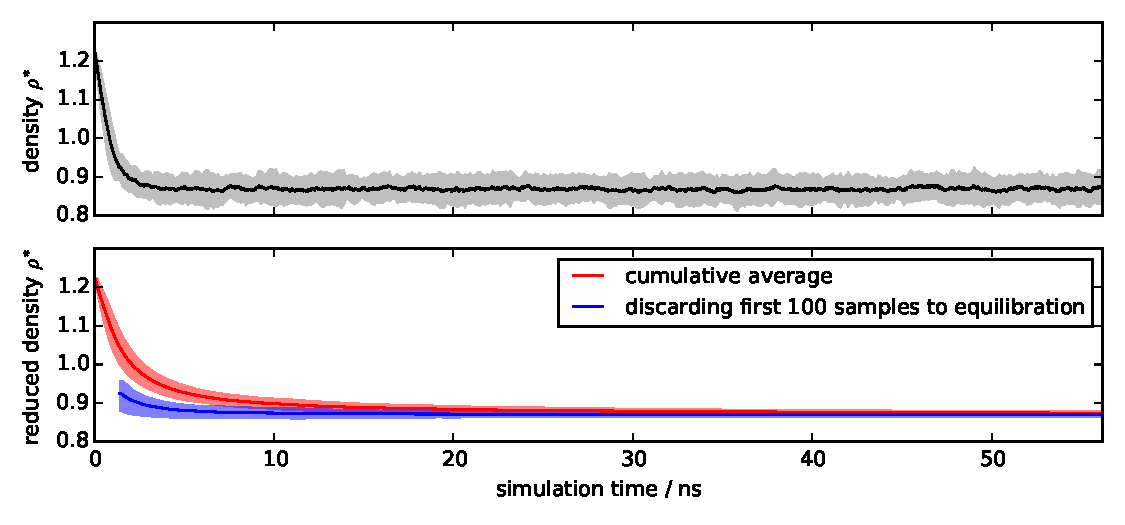
\includegraphics{argon-density.pdf}}
\caption{\label{figure:burn-in-example} {\bf Illustration of the motivation for discarding data to equilibration.} 
To illustrate the bias in expectations induced by relaxation away from initial conditions, 100 replicates of a simulation of liquid argon were initiated from the same energy-minimized initial configuration constructed with initial reduced density $\rho^* \equiv \rho \sigma^3 = 0.960$ but different random number seeds for stochastic integration.
%
{\bf Top:} The average of the reduced density (black line) over the replicates relaxes to the region of typical equilibrium densities over the first few ns of simulation time.
%
{\bf Bottom:} If the average density is estimated by a cumulative average from the beginning of the simulation (red line), the estimate will be heavily biased by the atypical starting density even beyond 10 ns.
Discarding even a small amount of initial data---in this case 100 initial samples (blue line)---results in a cumulative average estimate that converges to the true average (black dotted line) much more rapidly.
% 
Shaded regions denote 95\% confidence intervals.
%
Simulations were performed using a box of $N = 500$ argon atoms at reduced temperature $T^* \equiv k_B T / \epsilon = 0.850$ and reduced pressure $p^* \equiv p \sigma^3 / \epsilon = 1.266$ using a Langevin integrator~\cite{sivak-chodera-crooks:jpcb:2014:vvvr} with timestep $\Delta t = 0.01 \tau$, where characteristic oscillation timescale $\tau = \sqrt{m r_0^2 / 72 \epsilon}$, with $r_0 = 2^{1/6} \sigma$~\cite{liquid-argon-characteristic-timescale}.
A Metropolis Monte Carlo barostat was used with box volume moves attempted every 25 timesteps.
Densities were recorded every 25 timesteps.
}
\end{figure*}

%%%%%%%%%%%%%%%%%%%%%%%%%%%%%%%%%%%%%%%%%%%%%%%%%%%%%%%%%%%%%%%%%%%%%%%%%%%%%%%%
% STATISTICAL INEFFICIENCY
%%%%%%%%%%%%%%%%%%%%%%%%%%%%%%%%%%%%%%%%%%%%%%%%%%%%%%%%%%%%%%%%%%%%%%%%%%%%%%%%

\section*{Autocorrelation analysis}
\label{section:statistical-inefficiency}

The set of successively sampled configurations $\{x_t\}$ and their corresponding observables $\{a_t\}$ compose a correlated timeseries of observations.
To estimate the statistical error or uncertainty in a stationary timeseries free of bias, we must be able to quantify the \emph{effective number of uncorrelated samples} present in the dataset.
This is usually accomplished through computation of the \emph{statistical inefficiency} $g$, which quantifies the number of correlated timeseries samples needed to produce a single effectively uncorrelated sample of the observable of interest.
While this concept is well-established for the analysis of both Monte Carlo and molecular dynamics simulations~\cite{mueller-krumbhaar:j-stat-phys:1973:monte-carlo-analysis,swope:jcp:1982:autocorrelation-analysis,janke:2002:error-analysis,chodera:jctc:2007:wham}, we review it here for the sake of clarity.

For a given equilibration time choice $t_0$, the statistical uncertainty in our estimator $\hat{A}_{[t_0,T]}$ can be written as,
\begin{eqnarray}
\delta^2 \estimator{A}_{[t_0,T]} &\equiv& E_{x_0}\left[\left(\hat{A}_{[t_0,T]} - \expect{\estimator{A}}\right)^2\right] \nonumber \\
&=& E_{x_0}\left[ \hat{A}_{[t_0,T]} ^2 \right] - E_{x_0}\left[ \hat{A}_{[t_0,T]}  \right]^2 \nonumber \\
&=& \frac{1}{T_{t_0}^2} \sum_{t,t'=t_0}^T \left[ \expect{a_t a_{t'}} - \expect{a_t}\expect{a_{t'}} \right] \nonumber \\
&=& \frac{1}{T_{t_0}^2} \sum_{t=t_0}^T \left[ \expect{x_t^2} - \expect{x_t}^2 \right] \nonumber \\
\mbox{} &+& \frac{1}{T_{t_0}^2} \sum_{t\ne t' = t_0}^T \left[ \expect{a_t a_{t'}} - \expect{a_t}\expect{a_{t'}} \right] .
\end{eqnarray}
where $T_{t_0} \equiv T - t_0 + 1$, the number of correlated samples in the timeseries $\{a_t\}_{t_0}^T$.
In the last step, we have split the double-sum into two separate sums---a term capturing the variance in the observations $a_t$, and a remaining term capturing the correlation between observations. 

If $t_0$ is sufficiently large for the initial bias to be eliminated, the remaining timeseries $\{a_t\}_{t_0}^T$ will obey the properties of both \emph{stationarity} and \emph{time-reversibility}, allowing us to write,
\begin{eqnarray}
\lefteqn{\delta^2 \hat{A}_{[t_0,T]}^\mathrm{equil} = \frac{1}{T_{t_0}} \left[ \expect{a_t^2} - \expect{a_t}^2 \right]} \nonumber \\
\mbox{} &+& \frac{2}{T_{t_0}} \sum_{n=1}^{T-t_0} \left(\frac{T_{t_0}-n}{T_{t_0}}\right) \left[ \expect{a_t a_{t+n}} - \expect{a_t}\expect{a_{t+n}} \right]  \nonumber \\
&\equiv& \frac{\sigma_{t_0}^2}{T_{t_0}}(1 + 2 \tau_{t_0}) \nonumber \\
&=& \frac{\sigma_{t_0}^2}{T_{t_0}/g_{t_0}}
\end{eqnarray}
where the variance $\sigma^2$, statistical inefficiency $g$, and integrated autocorrelation time $\tau$ (in units of the sampling interval) are given by
\begin{eqnarray}
\sigma^2 &\equiv& \expect{a_t^2} - \expect{a_t}^2 \label{equation:variance-definition} \\
\tau &\equiv& \sum_{t=1}^{T-1} \left(1 - \frac{t}{T}\right) C_t \label{equation:integrated-autocorrelation-time-definition} \\
g &\equiv& 1 + 2 \tau \label{equation:statistical-inefficiency-definition}
\end{eqnarray}
with the discrete-time normalized fluctuation autocorrelation function $C_t$ defined as
\begin{eqnarray}
C_t &\equiv& \frac{\expect{a_n a_{n+t}} - \expect{a_n}^2}{\expect{a_n^2} - \expect{a_n}^2} . \label{equation:autocorrelation-definition}
\end{eqnarray}
In practice, it is difficult to estimate $C_t$ for $t \sim T$, due to growth in the statistical error, so common estimators of $g$ make use of several additional properties of $C_t$ to provide useful estimates~\cite{crc-mcmc-handbook}.

The $t_0$ subscript for the variance $\sigma^2$, the integrated autocorrelation time $\tau$, and the statistical inefficiency $t_0$ mean that these quantities are only estimated over the production portion of the timeseries, $\{a_t\}_{t=t_0}^T$.
Since we assumed that the bias was eliminated by judicious choice of the equilibration time $t_0$, this estimate of the statistical error will be poor for choices of $t_0$ that are too small.

%%%%%%%%%%%%%%%%%%%%%%%%%%%%%%%%%%%%%%%%%%%%%%%%%%%%%%%%%%%%%%%%%%%%%%%%%%%%%%%%
% THE IDEA
%%%%%%%%%%%%%%%%%%%%%%%%%%%%%%%%%%%%%%%%%%%%%%%%%%%%%%%%%%%%%%%%%%%%%%%%%%%%%%%%

\section*{The essential idea}
\label{section:the-idea}

Suppose we choose some arbitrary time $t_0$ and discard all samples $t \in [0, t_0)$ to equilibration, keeping $[t_0, T]$ as the dataset to analyze.
How much data remains?
We can determine this by computing the statistical inefficiency $g_{t_0}$ for the interval $[t_0, T]$, and computing the effective number of uncorrelated samples $N_\mathrm{eff}(t_0) \equiv (T - t_0 + 1) / g_{t_0}$.
If we start at $t_0 \equiv T$ and move $t_0$ to earlier and earlier points in time, we expect that the effective number of uncorrelated samples $N_\mathrm{eff}(t_0)$ will continue to grow until we start to include the highly atypical initial data.
At that point, the integrated autocorrelation time $\tau$ (and hence the statistical inefficiency $g$) will greatly increase, and the effective number of samples $N_\mathrm{eff}$ will start to plummet.


%%%%%%%%%%%%%%%%%%%%%%%%%%%%%%%%%%%%%%%%%%%%%%%%%%%%%%%%%%%%%%%%%%%%%%%%%%%%%%%%
% METHODS
%%%%%%%%%%%%%%%%%%%%%%%%%%%%%%%%%%%%%%%%%%%%%%%%%%%%%%%%%%%%%%%%%%%%%%%%%%%%%%%%

\section*{Illustration}
\label{section:methods}

Molecular dynamics simulations were performed with OpenMM 6.2~\cite{eastman:jctc:2012:openmm} using the Python API.
All scripts used to run simulations, analyze data, and generate plots---along with the simulation data itself---are availabile on GitHub at \url{http://github.com/choderalab/automatic-equilibration-detection}.
The automated equilibration detection scheme is also available in the \href{http://pymbar.readthedocs.org/en/latest/timeseries.html}{\tt timeseries} module of the \href{http://github.com/choderalab/pymbar}{\tt pymbar} package as {\tt detectEquilibration()}:
\begin{minted}[mathescape,
%               linenos,
               numbersep=5pt,
               gobble=0,
               frame=lines,
               framesep=2mm]{python}
from pymbar.timeseries import detectEquilibration
# determine equilibrated region
[t, g, Neff_max] = detectEquilibration(A_t)
# extract equilibrated region
A_t_equilibrated = A_t[t:]
\end{minted}

%%%%%%%%%%%%%%%%%%%%%%%%%%%%%%%%%%%%%%%%%%%%%%%%%%%%%%%%%%%%%%%%%%%%%%%%%%%%%%%%
% ACKNOWLEDGMENTS
%%%%%%%%%%%%%%%%%%%%%%%%%%%%%%%%%%%%%%%%%%%%%%%%%%%%%%%%%%%%%%%%%%%%%%%%%%%%%%%%

\section*{Acknowledgments}

We are grateful to William C.~Swope (IBM Almaden Research Center), Michael R.~Shirts (University of Virginia), David L.~Mobley (University of California, Irvine), Kyle A.~Beauchamp (MSKCC), and Robert C.~McGibbon (Stanford University) for valuable discussions on this topic, and Joshua L.~Adelman (University of Pittsburgh) for helpful feedback and encouragement.

%%%%%%%%%%%%%%%%%%%%%%%%%%%%%%%%%%%%%%%%%%%%%%%%%%%%%%%%%%%%%%%%%%%%%%%%%%%%%%%%
% BIBLIOGRAPHY
%%%%%%%%%%%%%%%%%%%%%%%%%%%%%%%%%%%%%%%%%%%%%%%%%%%%%%%%%%%%%%%%%%%%%%%%%%%%%%%%

\bibliographystyle{prsty} 
\bibliography{automatic-equilibration-detection}

\end{document}